\documentclass[a4paper, 14pt]{extarticle}

% Поля
%--------------------------------------
\usepackage{geometry}
\geometry{a4paper,tmargin=2cm,bmargin=2cm,lmargin=3cm,rmargin=1cm}
%--------------------------------------


%Russian-specific packages
%--------------------------------------
\usepackage[T2A]{fontenc}
\usepackage[utf8]{inputenc} 
\usepackage[english, main=russian]{babel}
%--------------------------------------

\usepackage{textcomp}

% Красная строка
%--------------------------------------
\usepackage{indentfirst}               
%--------------------------------------             


%Graphics
%--------------------------------------
\usepackage{graphicx}
\graphicspath{ {./images/} }
\usepackage{wrapfig}
%--------------------------------------

% Полуторный интервал
%--------------------------------------
\linespread{1.3}                    
%--------------------------------------

%Выравнивание и переносы
%--------------------------------------
% Избавляемся от переполнений
\sloppy
% Запрещаем разрыв страницы после первой строки абзаца
\clubpenalty=10000
% Запрещаем разрыв страницы после последней строки абзаца
\widowpenalty=10000
%--------------------------------------

%Списки
\usepackage{enumitem}

%Подписи
\usepackage{caption} 

%Гиперссылки
\usepackage{hyperref}

\hypersetup {
	unicode=true
}

%Рисунки
%--------------------------------------
\DeclareCaptionLabelSeparator*{emdash}{~--- }
\captionsetup[figure]{labelsep=emdash,font=onehalfspacing,position=bottom}
%--------------------------------------

\usepackage{tempora}

%Листинги
%--------------------------------------
\usepackage{listings}
\lstset{
  basicstyle=\ttfamily\footnotesize, 
  %basicstyle=\footnotesize\AnkaCoder,        % the size of the fonts that are used for the code
  breakatwhitespace=false,         % sets if automatic breaks shoulbd only happen at whitespace
  breaklines=true,                 % sets automatic line breaking
  captionpos=t,                    % sets the caption-position to bottom
  inputencoding=utf8,
  frame=single,                    % adds a frame around the code
  keepspaces=true,                 % keeps spaces in text, useful for keeping indentation of code (possibly needs columns=flexible)
  keywordstyle=\bf,       % keyword style
  numbers=left,                    % where to put the line-numbers; possible values are (none, left, right)
  numbersep=5pt,                   % how far the line-numbers are from the code
  xleftmargin=25pt,
  xrightmargin=25pt,
  showspaces=false,                % show spaces everywhere adding particular underscores; it overrides 'showstringspaces'
  showstringspaces=false,          % underline spaces within strings only
  showtabs=false,                  % show tabs within strings adding particular underscores
  stepnumber=1,                    % the step between two line-numbers. If it's 1, each line will be numbered
  tabsize=2,                       % sets default tabsize to 8 spaces
  title=\lstname                   % show the filename of files included with \lstinputlisting; also try caption instead of title
}
%--------------------------------------

%%% Математические пакеты %%%
%--------------------------------------
\usepackage{amsthm,amsfonts,amsmath,amssymb,amscd}  % Математические дополнения от AMS
\usepackage{mathtools}                              % Добавляет окружение multlined
\usepackage[perpage]{footmisc}
%--------------------------------------

%--------------------------------------
%			НАЧАЛО ДОКУМЕНТА
%--------------------------------------

\begin{document}

%--------------------------------------
%			ТИТУЛЬНЫЙ ЛИСТ
%--------------------------------------
\begin{titlepage}
\thispagestyle{empty}
\newpage


%Шапка титульного листа
%--------------------------------------
\vspace*{-60pt}
\hspace{-65pt}
\begin{minipage}{0.3\textwidth}
\hspace*{-20pt}\centering

\includegraphics[width=\textwidth]{emblem}
\end{minipage}
\begin{minipage}{0.67\textwidth}\small \textbf{
\vspace*{-0.7ex}
\hspace*{-6pt}\centerline{Министерство науки и высшего образования Российской Федерации}
\vspace*{-0.7ex}
\centerline{Федеральное государственное бюджетное образовательное учреждение }
\vspace*{-0.7ex}
\centerline{высшего образования}
\vspace*{-0.7ex}
\centerline{<<Московский государственный технический университет}
\vspace*{-0.7ex}
\centerline{имени Н.Э. Баумана}
\vspace*{-0.7ex}
\centerline{(национальный исследовательский университет)>>}
\vspace*{-0.7ex}
\centerline{(МГТУ им. Н.Э. Баумана)}}
\end{minipage}
%--------------------------------------

%Полосы
%--------------------------------------
\vspace{-25pt}
\hspace{-35pt}\rule{\textwidth}{2.3pt}

\vspace*{-20.3pt}
\hspace{-35pt}\rule{\textwidth}{0.4pt}
%--------------------------------------

\vspace{1.5ex}
\hspace{-35pt} \noindent \small ФАКУЛЬТЕТ\hspace{80pt} <<Информатика и системы управления>>

\vspace*{-16pt}
\hspace{47pt}\rule{0.83\textwidth}{0.4pt}

\vspace{0.5ex}
\hspace{-35pt} \noindent \small КАФЕДРА\hspace{50pt} <<Теоретическая информатика и компьютерные технологии>>

\vspace*{-16pt}
\hspace{30pt}\rule{0.866\textwidth}{0.4pt}
  
\vspace{11em}

\begin{center}
\Large {\bf Контрольная работа № 2.1} \\
\large {\bf по курсу <<Разработка мобильных приложений>>} \\
\large <<Калькулятор на Kotlin>>
\end{center}\normalsize

\vspace{8em}


\begin{flushright}
  {Студентка группы ИУ9-72Б Самохвалова П. С. \hspace*{15pt}\\
  \vspace{2ex}
  Преподаватель Посевин Д. П.\hspace*{15pt}}
\end{flushright}

\bigskip

\vfill
 

\begin{center}
\textsl{Москва 2023}
\end{center}
\end{titlepage}
%--------------------------------------
%		КОНЕЦ ТИТУЛЬНОГО ЛИСТА
%--------------------------------------

\renewcommand{\ttdefault}{pcr}

\setlength{\tabcolsep}{3pt}
\newpage
\setcounter{page}{2}

\section{Задание}\label{Sect::task}

Реализовать калькулятор разобранный на лекции, но расширив его дополнительным функционалом в зависимости от варианта с использованием Expression Builder. Например, расчет тригонометрических функций, логических выражений и т. д.

Индивидуальный вариант:

exponentation: $2^2$

cbrt: cubic root

cosh: hyperbolic cosine

\section{Практическая реализация}\label{Sect::code}

Исходный код программы представлен в листинге~\ref{lst:code1}.

\begin{lstlisting}[language={},caption={Калькулятор на Kotlin},label={lst:code1}]
package com.example.calculator


//import kotlinx.android.synthetic.main.activity_main.*
import android.annotation.SuppressLint
import android.os.Bundle
import android.widget.TextView
import androidx.appcompat.app.AppCompatActivity
import net.objecthunter.exp4j.ExpressionBuilder

class MainActivity : AppCompatActivity()
{

    @SuppressLint("MissingInflatedId")
    override fun onCreate(savedInstanceState: Bundle?) {
        super.onCreate(savedInstanceState)
        setContentView(R.layout.activity_main)


        /*Number Buttons*/
        val tvExpression: TextView = findViewById(R.id.tvExpression)

        val tvOne: TextView = findViewById(R.id.tvOne)
        tvOne.setOnClickListener {
            tvExpression.text = tvExpression.text.toString() + "1"
        }

        val tvTwo: TextView = findViewById(R.id.tvTwo)
        tvTwo.setOnClickListener {
            tvExpression.text = tvExpression.text.toString() + "2"
        }

        val tvThree: TextView = findViewById(R.id.tvThree)
        tvThree.setOnClickListener {
            tvExpression.text = tvExpression.text.toString() + "3"
        }

        val tvFour: TextView = findViewById(R.id.tvFour)
        tvFour.setOnClickListener {
            tvExpression.text = tvExpression.text.toString() + "4"
        }

        val tvFive: TextView = findViewById(R.id.tvFive)
        tvFive.setOnClickListener {
            tvExpression.text = tvExpression.text.toString() + "5"
        }

        val tvSix: TextView = findViewById(R.id.tvSix)
        tvSix.setOnClickListener {
            tvExpression.text = tvExpression.text.toString() + "6"
        }

        val tvSeven: TextView = findViewById(R.id.tvSeven)
        tvSeven.setOnClickListener {
            tvExpression.text = tvExpression.text.toString() + "7"
        }

        val tvEight: TextView = findViewById(R.id.tvEight)
        tvEight.setOnClickListener {
            tvExpression.text = tvExpression.text.toString() + "8"
        }

        val tvNine: TextView = findViewById(R.id.tvNine)
        tvNine.setOnClickListener {
            tvExpression.text = tvExpression.text.toString() + "9"
        }

        val tvZero: TextView = findViewById(R.id.tvZero)
        tvZero.setOnClickListener {
            tvExpression.text = tvExpression.text.toString() + "0"
        }

        /*Operators*/

        val tvPlus: TextView = findViewById(R.id.tvPlus)
        tvPlus.setOnClickListener {
            tvExpression.text = tvExpression.text.toString() + "+"
        }

        val tvMinus: TextView = findViewById(R.id.tvMinus)
        tvMinus.setOnClickListener {
            tvExpression.text = tvExpression.text.toString() + "-"
        }

        val tvMul: TextView = findViewById(R.id.tvMul)
        tvMul.setOnClickListener {
            tvExpression.text = tvExpression.text.toString() + "*"
        }

        val tvDivide: TextView = findViewById(R.id.tvDivide)
        tvDivide.setOnClickListener {
            tvExpression.text = tvExpression.text.toString() + "/"
        }

        val tvDot: TextView = findViewById(R.id.tvDot)
        tvDot.setOnClickListener {
            tvExpression.text = tvExpression.text.toString() + "."
        }

        val tvDeg: TextView = findViewById(R.id.tvDeg)
        tvDeg.setOnClickListener {
            tvExpression.text = tvExpression.text.toString() + "^"
        }

        val tvRoot: TextView = findViewById(R.id.tvRoot)
        tvRoot.setOnClickListener {
            tvExpression.text = "cbrt(" + tvExpression.text.toString() + ")"
        }

        val tvCosh: TextView = findViewById(R.id.tvCosh)
        tvCosh.setOnClickListener {
            tvExpression.text = "cosh(" + tvExpression.text.toString() + ")"
        }

        val tvClear: TextView = findViewById(R.id.tvClear)

        val tvResult: TextView = findViewById(R.id.tvResult)
        tvClear.setOnClickListener {
            tvExpression.text = ""
            tvResult.text = ""
        }

        val tvEquals: TextView = findViewById(R.id.tvEquals)
        tvEquals.setOnClickListener {
            val text = tvExpression.text.toString()
            val expression = ExpressionBuilder(text).build()

            val result = expression.evaluate()
            val longResult = result.toLong()
            if (result == longResult.toDouble()) {
                tvResult.text = longResult.toString()
            } else {
                tvResult.text = result.toString()
            }
        }
        val tvBack: TextView = findViewById(R.id.tvBack)
        tvBack.setOnClickListener {
            val text = tvExpression.text.toString()
            if(text.isNotEmpty()) {
                tvExpression.text = text.drop(1)
            }

            tvResult.text = ""
        }
    }

}

<?xml version="1.0" encoding="utf-8"?>
<LinearLayout xmlns:android="http://schemas.android.com/apk/res/android"
    xmlns:app="http://schemas.android.com/apk/res-auto"
    xmlns:tools="http://schemas.android.com/tools"
    android:layout_width="match_parent"
    android:layout_height="match_parent"
    tools:context=".MainActivity"
    android:background="@android:color/black"
    android:orientation="vertical">

    <TextView
        android:id="@+id/tvExpression"
        android:layout_width="match_parent"
        android:layout_height="80dp"
        android:textColor="@color/actionButton"
        android:layout_gravity="end"
        android:ellipsize="start"
        android:singleLine="true"
        android:textSize="40sp" />


    <TextView
        android:id="@+id/tvResult"
        android:layout_width="match_parent"
        android:layout_height="100dp"
        android:textColor="@color/white"
        android:layout_gravity="end"
        android:ellipsize="end"
        android:singleLine="true"
        android:textSize="30sp"/>


    <LinearLayout
        android:layout_width="match_parent"
        android:layout_height="match_parent"
        android:orientation="vertical">

        <LinearLayout
            android:layout_width="match_parent"
            android:layout_height="0dp"
            android:layout_weight="1"
            android:orientation="horizontal">
            <TextView
                android:id="@+id/tvClear"
                style="@style/ActionButtonStyle"
                android:text="CLEAR"/>

            <TextView
                android:id="@+id/tvDivide"
                style="@style/ActionButtonStyle"
                android:text="/"/>


        </LinearLayout>

        <LinearLayout
            android:layout_width="match_parent"
            android:layout_height="0dp"
            android:layout_weight="1"
            android:orientation="horizontal">

            <TextView
                android:id="@+id/tvSeven"
                style="@style/NumberButtonStyle"
                android:text="7"/>

            <TextView
                android:id="@+id/tvEight"
                style="@style/NumberButtonStyle"
                android:text="8"/>

            <TextView
                android:id="@+id/tvNine"
                style="@style/NumberButtonStyle"
                android:text="9"/>

            <TextView
                android:id="@+id/tvMul"
                style="@style/NumberActionButton2"
                android:text="*"/>

            <TextView
                android:id="@+id/tvDeg"
                style="@style/NumberActionButton2"
                android:text="^"/>

        </LinearLayout>

        <LinearLayout
            android:layout_width="match_parent"
            android:layout_height="0dp"
            android:layout_weight="1"
            android:orientation="horizontal">

            <TextView
                android:id="@+id/tvFour"
                style="@style/NumberButtonStyle"
                android:text="4"/>

            <TextView
                android:id="@+id/tvFive"
                style="@style/NumberButtonStyle"
                android:text="5"/>

            <TextView
                android:id="@+id/tvSix"
                style="@style/NumberButtonStyle"
                android:text="6"/>

            <TextView
                android:id="@+id/tvMinus"
                style="@style/NumberActionButton2"
                android:text="-"/>

            <TextView
                android:id="@+id/tvRoot"
                style="@style/NumberActionButton2"
                android:text="cbrt"/>


        </LinearLayout>

        <LinearLayout
            android:layout_width="match_parent"
            android:layout_height="0dp"
            android:layout_weight="1"
            android:orientation="horizontal">

            <TextView
                android:id="@+id/tvOne"
                style="@style/NumberButtonStyle"
                android:text="1"/>

            <TextView
                android:id="@+id/tvTwo"
                style="@style/NumberButtonStyle"
                android:text="2"/>

            <TextView
                android:id="@+id/tvThree"
                style="@style/NumberButtonStyle"
                android:text="3"/>

            <TextView
                android:id="@+id/tvPlus"
                style="@style/NumberActionButton2"
                android:text="+"/>

            <TextView
                android:id="@+id/tvCosh"
                style="@style/NumberActionButton2"
                android:text="cosh"/>


        </LinearLayout>

        <LinearLayout
            android:layout_width="match_parent"
            android:layout_height="0dp"
            android:layout_weight="1"
            android:orientation="horizontal">

            <TextView
                android:id="@+id/tvDot"
                style="@style/NumberButtonStyle"
                android:text="."/>

            <TextView
                android:id="@+id/tvZero"
                style="@style/NumberButtonStyle"
                android:text="0"/>

            <TextView
                android:id="@+id/tvBack"
                style="@style/NumberButtonStyle"
                android:text="DEL"/>

            <TextView
                android:id="@+id/tvEquals"
                style="@style/EqualButtonStyle"
                android:text="="/>


        </LinearLayout>

    </LinearLayout>


</LinearLayout>
\end{lstlisting}

\section{Результаты}\label{Sect::res}

Результаты работы программы представлены на рисунках~\ref{fig:img1}~--~\ref{fig:img3}.

\begin{figure}[!htb]
	\centering
	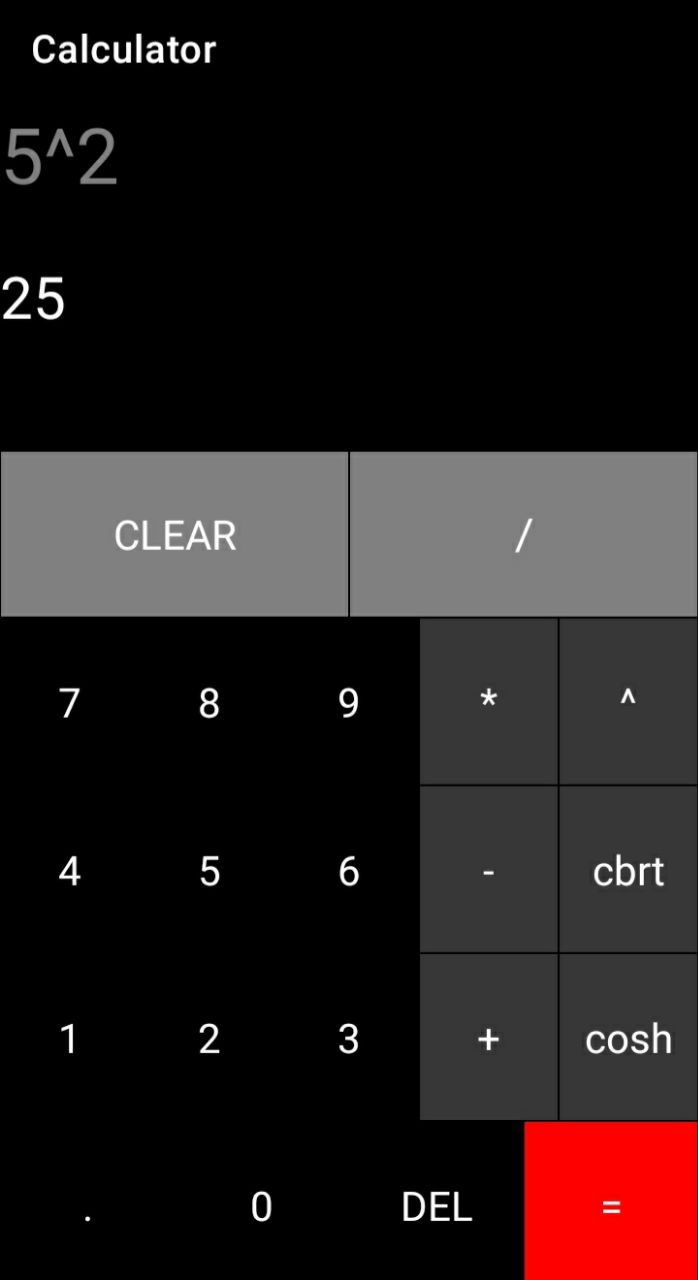
\includegraphics[width=0.8\textwidth]{img1}
\caption{Возведение в степень}
\label{fig:img1}
\end{figure}

\begin{figure}[!htb]
	\centering
	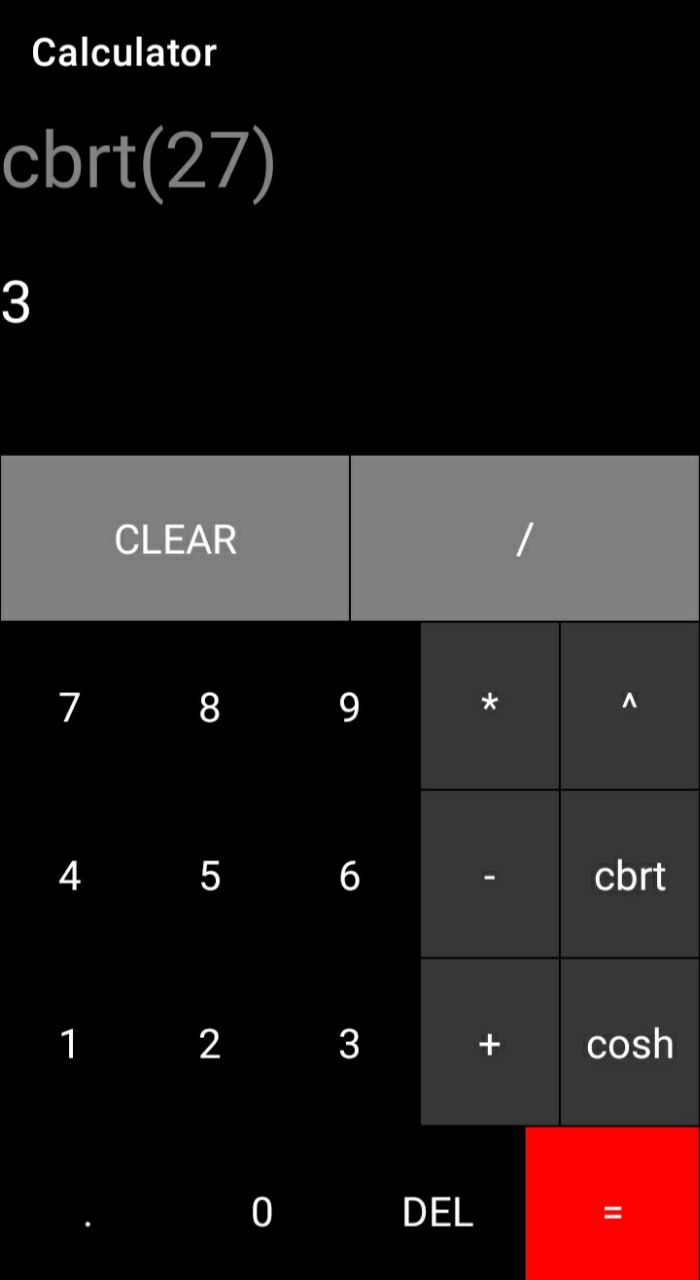
\includegraphics[width=0.8\textwidth]{img2}
\caption{Кубический корень}
\label{fig:img2}
\end{figure}

\begin{figure}[!htb]
	\centering
	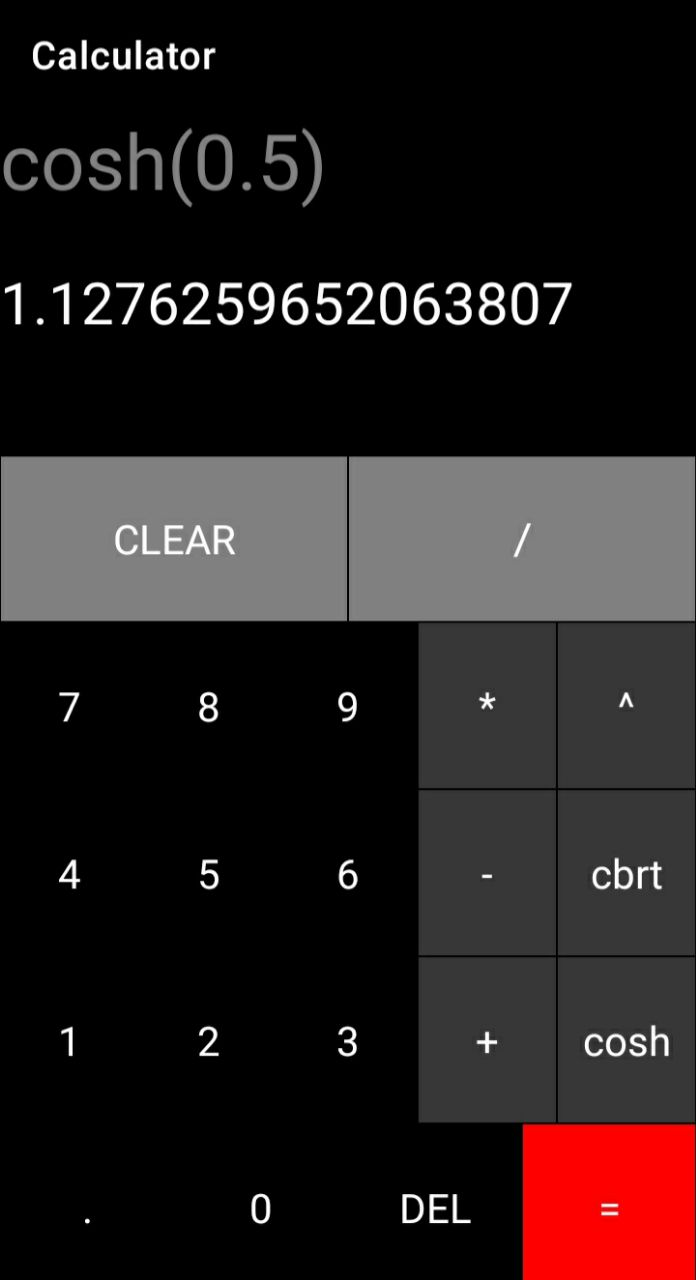
\includegraphics[width=0.8\textwidth]{img3}
\caption{Гиперболический косинус}
\label{fig:img3}
\end{figure}

\section{Выводы}\label{Sect::conclusion}

В результате выполнения рубежного контроля калькулятор был дополнен возведением в степень, вычислением кубического корня и гиперболического косинуса.

\end{document}
